 % !TeX root = ../main.tex
\documentclass[../main.tex]{subfiles}
\begin{document}
\section{Konkrete Zahlen}
Hier werden die hergeleiteten Formeln angewendet um konkrete Zahlen zu erhalten. Um einen Maßstab zu sehen werden jeweils ein Erdenjahr (365 Tage) ein Marsjahr (780 Tage) und ein Jupiterjahr (4330 Tage) gezeigt.
\subsection{Wahrscheinlichkeit der ersten Kollision}

Mithilfe der Formel \ref{num.pleq} wird die Wahrscheinlichkeiten dafür berechnet, dass $X \leq k$ ist. X ist hierbei der Zeitpunkt der 1. Kollision. Mit der Formel \ref{num.peq} wird die Wahrscheinlichkeit erechnet, dass die Kollision bei K stattfindet.

\begin{equation}
 P(X \leq k) \approx 1 - e^{- \frac{k(k-1)}{2n}}
 \label{num.pleq}
\end{equation}

\begin{equation}
 P(X = k) \approx \frac{(k-1)}{n} \cdot e^{- \frac{(k-1)^2}{2n}}
 \label{num.peq}
\end{equation}

\subsubsection{$P(X \leq k)$}

\textbf{Erde}

\begin{table}[h]
\centering
\begin{tabular}{l|l|l|l}
k  & $P(X_{n}) \leq k)$ & k  & $P(X_{n}) \leq k)$ \\ \hline
0  & 0,001            & 40 & 0,876            \\
10 & 0,105            & 50 & 0,963            \\
20 & 0,390            & 60 & 0,992            \\
30 & 0,684            & 70 & 0,999
\end{tabular}
\end{table}

\begin{figure}[h]
 \begin{center}
 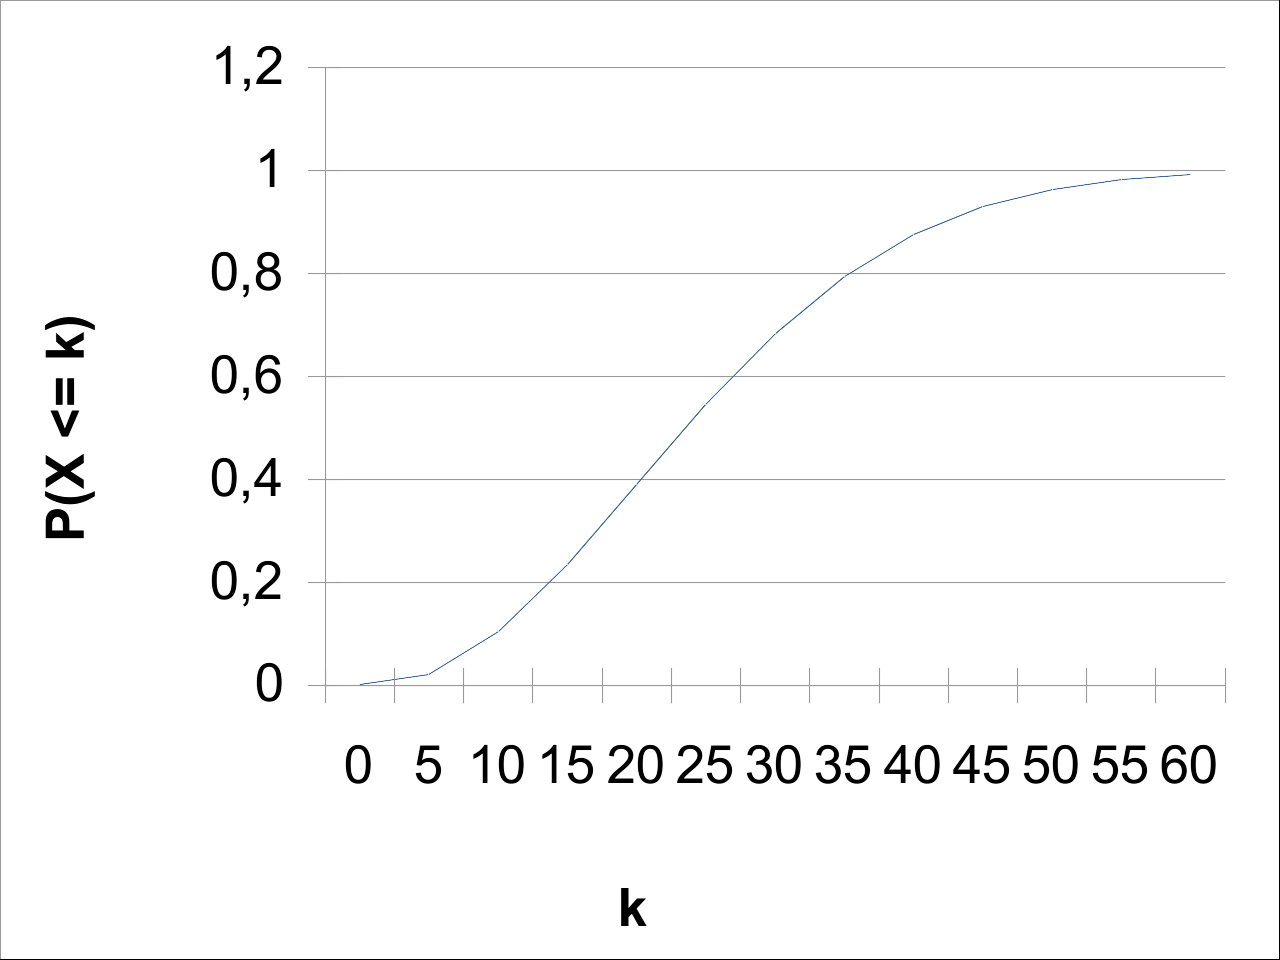
\includegraphics[width=0.7\textwidth]{../graphics/perde.png}
 % qerde.png: 1280x960 px, 72dpi, 45.16x33.87 cm, bb=0 0 1280 960
\end{center}

\end{figure}


\textbf{Mars}

\begin{table}[h]
\centering
\begin{tabular}{l|l|l|l|}
k  & $P(X_{n} \leq k)$ & k  & $P(X_{n} \leq k)$ \\ \hline
0  & 0,001            & 60 & 0,893            \\
15 & 0,118            & 75 & 0,970            \\
30 & 0,417            & 90 & 0,994            \\
45 & 0,711            &    &
\end{tabular}
\end{table}

\textbf{Jupiter}

\begin{table}[h]
\centering
\begin{tabular}{l|l|l|l|}
k  & $P(X_{n} \leq k)$ & k   & $P(X_{n} \leq k)$\\ \hline
0  & 0                & 120 & 0,805            \\
30 & 0,093            & 150 & 0,923            \\
60 & 0,331            & 180 & 0,975            \\
90 & 0,599            & 210 & 0,994
\end{tabular}
\end{table}

\subsubsection{$P(X = k)$}

\textbf{Erde}

\begin{table}[h]
\centering
\begin{tabular}{l|l|l|l|l|l}
k  & $P(X_{n} = k)$ & k  & $P(X_{n} = k)$ & k  & $P(X_{n} = k)$ \\ \hline
5  & 0,011            & 25 & 0,030            & 45 & 0,009            \\
10 & 0,022            & 30 & 0,025            & 50 & 0,005            \\
15 & 0,029            & 35 & 0,019            & 55 & 0,003            \\
20 & 0,032            & 40 & 0,013            & 60 & 0,001
\end{tabular}
\end{table}

\begin{center}
 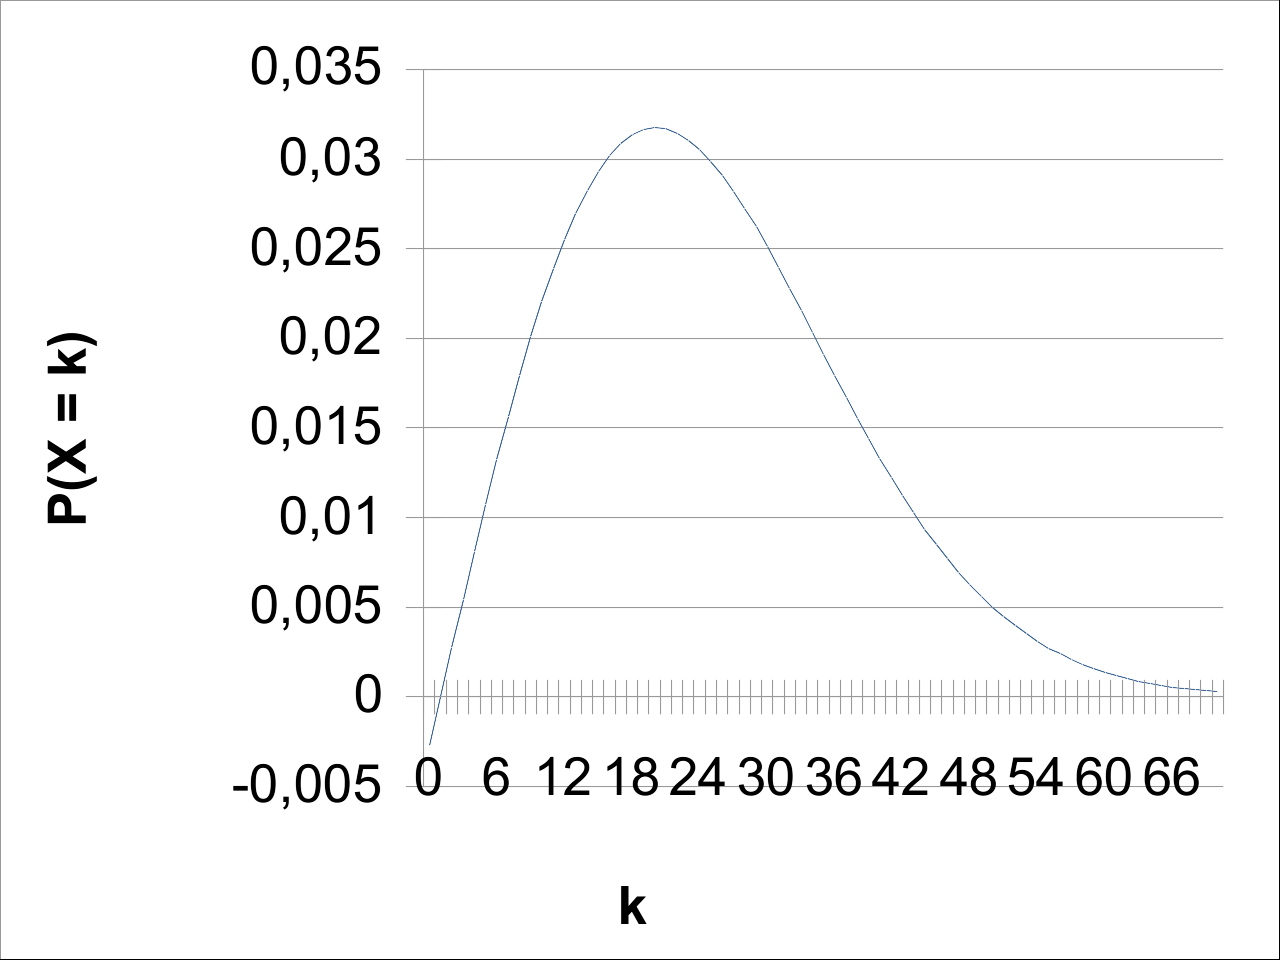
\includegraphics[width=0.7\textwidth]{../graphics/peq.png}
 % peq.png: 1280x960 px, 72dpi, 45.16x33.87 cm, bb=0 0 1280 960
\end{center}

Die höchste Wahrscheinlichkeit dafür, dass die 1. Kollision genau bei k auftritt liegt auf der Erde bei \bm{$\sim 20,105$}, auf dem Mars bei \bm{$\sim 28,928$} und auf dem Jupiter bei \bm{$\sim 66,803$} also jeweils bei \bm{$1 + \sqrt{n}$}.

\subsection{Erwartungswerte}

Der Erwartungswert für die 1. Kollision wird über die Formel \ref{num.exp} errechnet.

\begin{equation}
 E(X) \approx 1 + \sqrt{\frac{1}{2} \pi n}
 \label{num.exp}
\end{equation}

Für die verschiedenen Planeten kommen dabei folgende Werte heraus:

\begin{center}
\begin{tabular}{l|l}
Erde & 24,945\\ \hline
Mars & 36,003\\ \hline
Jupiter & 83,472
\end{tabular}
\end{center}

\subsection{Quantile}

Die Quantile für die 1. Kollision werden über die Formel

\begin{equation}
 q_{\alpha} \approx 1 + \sqrt{-n ln(1-\alpha)}
\end{equation}



\end{document}
